\subsection{Loss History}
    Following are the loss vs iteration graphs. First plot compares ACMR\cite{acmr} and OCMFH\cite{ocmfh} on nuswide dataset. Remaining graphs are for OCMFH\cite{ocmfh} algorithm for varying bit length on both nuswide and xmedianet dataset.
        \begin{figure}[H]
            \begin{minipage}[!h]{0.6\linewidth}
                \centering
                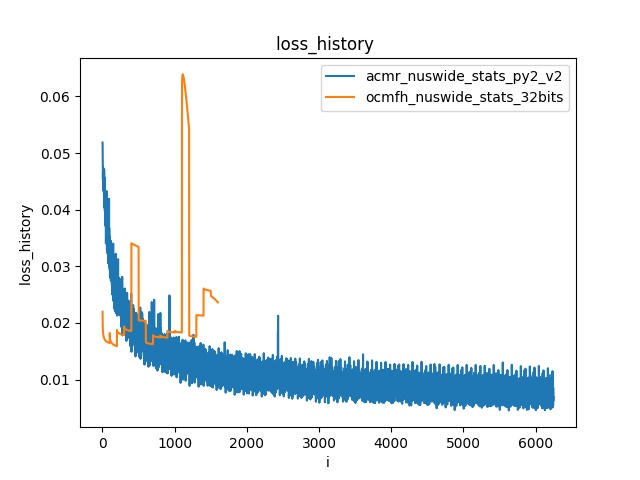
\includegraphics[width=\linewidth]{resultsImages/lossHistory/loss_history_both_nuswide.jpeg}
                % \caption{Inter comparison(NUS-WIDE)}
                % \label{fig:}
                \vspace{0.1ex}
                \hspace{0.1ex}
            \end{minipage}
            \begin{minipage}[!h]{0.6\linewidth}
                \centering
                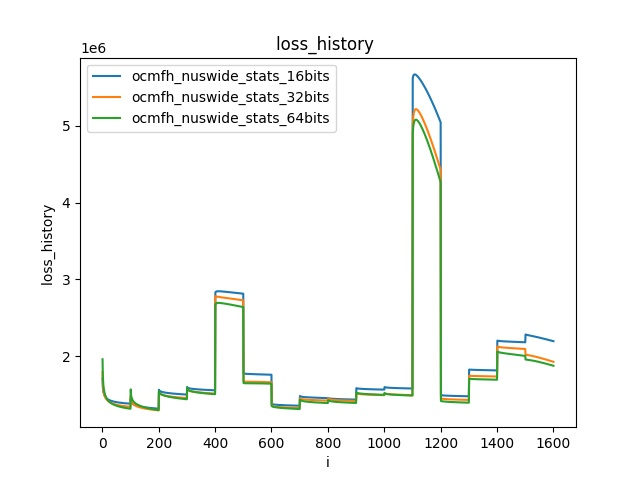
\includegraphics[width=\linewidth]{resultsImages/lossHistory/loss_history_ocmfh_nuswide_bits.jpeg}
                % \caption{OCMFH changing bits(NUS-WIDE)}
                % \label{fig:}
                \vspace{0.1ex}
                \hspace{0.1ex}
            \end{minipage}
            \begin{minipage}[!h]{0.7\linewidth}
                \centering
                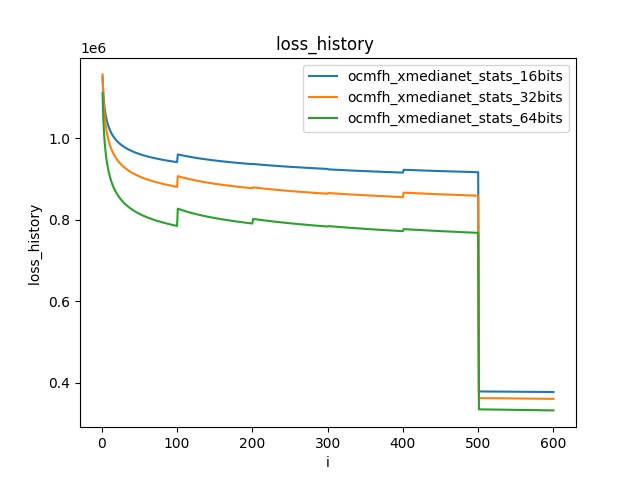
\includegraphics[width=\linewidth]{resultsImages/lossHistory/loss_history_ocmfh_xmedianet_bits.jpeg}
                % \caption{OCMFH chaning bits(Xmedianet)}
                % \label{fig:}
                \vspace{0.1ex}
                \hspace{1ex}
            \end{minipage}
            \caption{Loss vs iteration graph for inter and intra method comparison}
        \label{fig:}
        \end{figure}
        \FloatBarrier